\documentclass[a4paper,12pt]{article}

\usepackage[utf8]{inputenc}
\usepackage{geometry}
\usepackage{graphicx}
\usepackage{amsmath}
\usepackage{hyperref}

\geometry{margin=1in}

\title{MatLab 1}
\author{B13901165張勝勛 \\ 班級：王鈺強老師班}
\date{\today}

% Language and font packages
\usepackage{ctex} % Chinese support

% Pseudocode and algorithm packages
% \usepackage{algorithm2e} % Advanced algorithm writing
% \usepackage{algpseudocode} % Pseudocode environment for algorithms

% Fancy style packages
\usepackage{fancyhdr} % Custom headers/footers
\usepackage{color} % Color support
\usepackage{xcolor} % Extended color support
\usepackage{tcolorbox} % Colored boxes
\usepackage{framed} % Framed environments

% Math and symbol packages
\usepackage{amsfonts}
\usepackage{amssymb}
\usepackage{mathtools}

% Table and figure packages
% \usepackage{booktabs} % Professional tables
% \usepackage{multirow} % Multi-row tables
% \usepackage{caption} % Custom captions
\usepackage{subcaption} % Subfigures

% Miscellaneous
\usepackage{enumitem} % Custom lists
\usepackage{listings} % Code listings
\usepackage{tikz} % Drawing diagrams
\usepackage{pgfplots} % For plotting graphs
\usepackage{float}

\begin{document}

\maketitle

\section{Matlab result}
\begin{figure}[H]
    \centering
    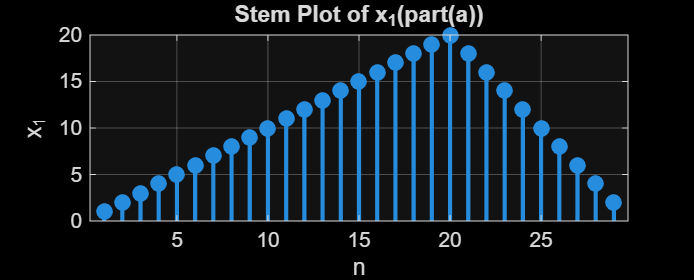
\includegraphics[width=0.85\textwidth]{Figure-1.png}
    \caption{The result for Part(A)}
    \label{fig:example}
\end{figure}

\begin{figure}[H]
    \centering
    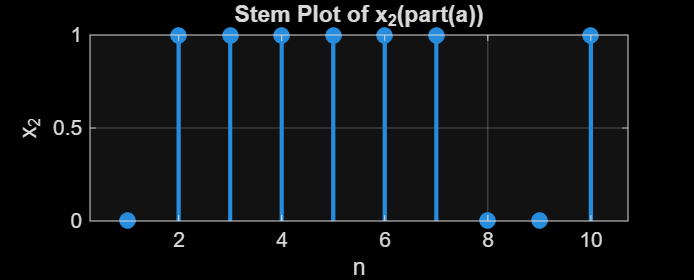
\includegraphics[width=0.85\textwidth]{Figure-2.png}
    \caption{The result for Part(A)}
    \label{fig:example}
\end{figure}

\begin{figure}[H]
    \centering
    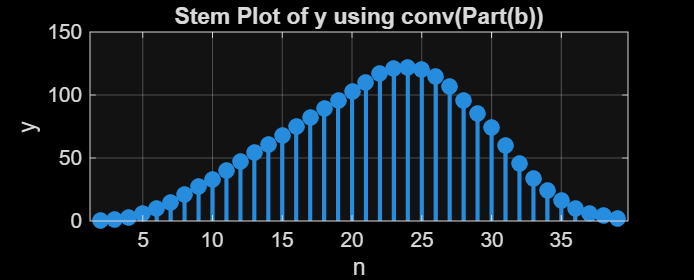
\includegraphics[width=0.85\textwidth]{Figure-3.png}
    \caption{The result for Part(B)}
    \label{fig:example}
\end{figure}
\begin{figure}[H]
    \centering
    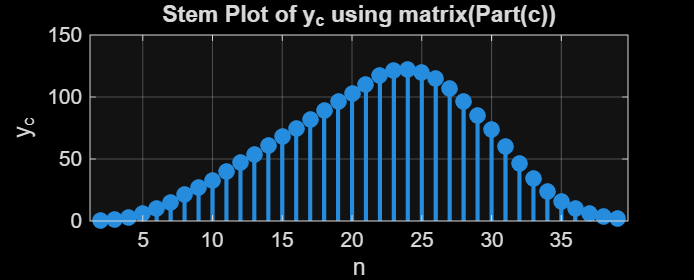
\includegraphics[width=0.85\textwidth]{Figure-4.png}
    \caption{The result for Part(C)}
    \label{fig:example}
\end{figure}

\begin{figure}[H]
    \centering
    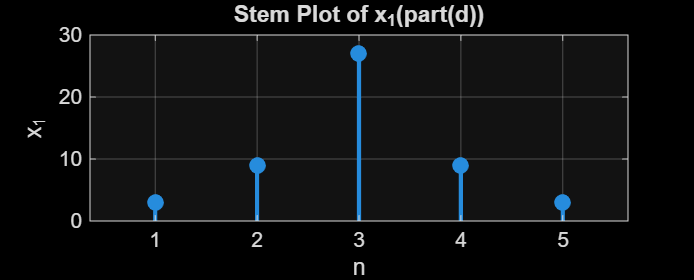
\includegraphics[width=0.85\textwidth]{Figure-5.png}
    \caption{The result for Part(D)}
    \label{fig:example}
\end{figure}
\begin{figure}[H]
    \centering
    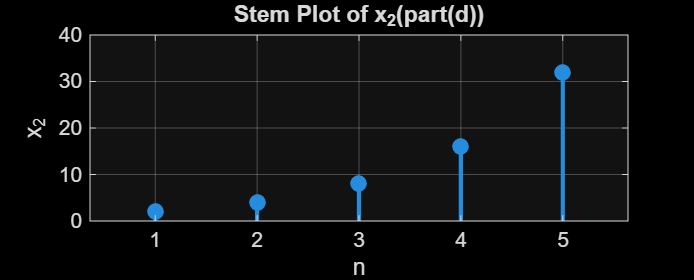
\includegraphics[width=0.85\textwidth]{Figure-6.png}
    \caption{The result for Part(D)}
    \label{fig:example}
\end{figure}
\begin{figure}[H]
    \centering
    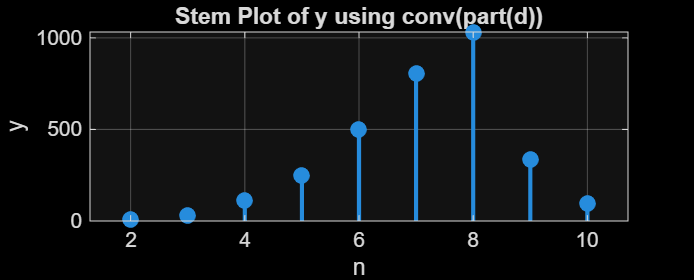
\includegraphics[width=0.85\textwidth]{Figure-7.png}
    \caption{The result for Part(D)}
    \label{fig:example}
\end{figure}
\begin{figure}[H]
    \centering
    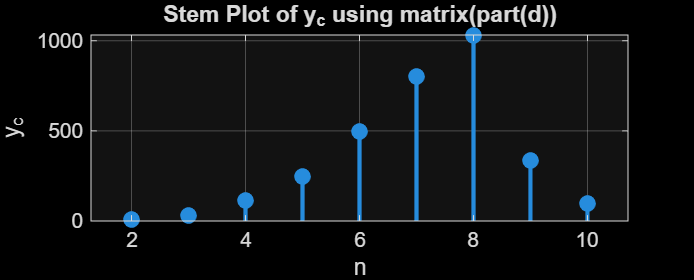
\includegraphics[width=0.85\textwidth]{Figure-8.png}
    \caption{The result for Part(D)}
    \label{fig:example}
\end{figure}

\newpage

\section{Part(C) code implementation}
\begin{lstlisting}[language=matlab, caption=MATLAB Code, basicstyle=\ttfamily\small, breaklines=true, frame=single]
%%part(c)
N1 = length(x_1);
N2 = length(x_2);

col = [x_1, zeros(1, N2-1)];
row = [x_1(1), zeros(1, N2-1)];
matrix = toeplitz(col, row);
y_c = matrix * x_2';

if isequal(round(y_c, 5), round(y', 5))
    disp('The result is the same');
end

figure;
stem(n_y, y_c, "filled", "LineWidth", 2);
title('Stem Plot of y_c using matrix(Part(c))');
xlabel('n'); ylabel('y_c');
grid on;
\end{lstlisting}

\end{document}